\begin{enumerate}[label=\thesubsection.\arabic*.,ref=\thesubsection.\theenumi]
\numberwithin{equation}{enumi}
\item Using the frequency response method, design a lag-lead compensator for the unity feedback system given 
\begin{align}
G(S) = \frac{K(s+7)}{s(s+5)(s+15)}
\end{align}
The following specifications must be met: Peak overshoot = 15\%, settling time = 0.1 second and velocity error constant = 1000
Use second order approximation. \\
%
\solution Figure: \ref{fig:1;} models the equivalent of compensated closed loop system. 
\begin{figure}[!ht]
\begin{center}
		\resizebox{\columnwidth}{!}{\begin{enumerate}[label=\thesubsection.\arabic*.,ref=\thesubsection.\theenumi]
\numberwithin{equation}{enumi}
\item Using the frequency response method, design a lag-lead compensator for the unity feedback system given 
\begin{align}
G(S) = \frac{K(s+7)}{s(s+5)(s+15)}
\end{align}
The following specifications must be met: Peak overshoot = 15\%, settling time = 0.1 second and velocity error constant = 1000
Use second order approximation. \\
%
\solution Figure: \ref{fig:1;} models the equivalent of compensated closed loop system. 
\begin{figure}[!ht]
\begin{center}
		\resizebox{\columnwidth}{!}{\begin{enumerate}[label=\thesubsection.\arabic*.,ref=\thesubsection.\theenumi]
\numberwithin{equation}{enumi}
\item Using the frequency response method, design a lag-lead compensator for the unity feedback system given 
\begin{align}
G(S) = \frac{K(s+7)}{s(s+5)(s+15)}
\end{align}
The following specifications must be met: Peak overshoot = 15\%, settling time = 0.1 second and velocity error constant = 1000
Use second order approximation. \\
%
\solution Figure: \ref{fig:1;} models the equivalent of compensated closed loop system. 
\begin{figure}[!ht]
\begin{center}
		\resizebox{\columnwidth}{!}{\begin{enumerate}[label=\thesubsection.\arabic*.,ref=\thesubsection.\theenumi]
\numberwithin{equation}{enumi}
\item Using the frequency response method, design a lag-lead compensator for the unity feedback system given 
\begin{align}
G(S) = \frac{K(s+7)}{s(s+5)(s+15)}
\end{align}
The following specifications must be met: Peak overshoot = 15\%, settling time = 0.1 second and velocity error constant = 1000
Use second order approximation. \\
%
\solution Figure: \ref{fig:1;} models the equivalent of compensated closed loop system. 
\begin{figure}[!ht]
\begin{center}
		\resizebox{\columnwidth}{!}{\input{./figs/ee18btech11012/ee18btech11012_1.tex}}
\end{center}
\caption{}
\label{fig:ee18btech11012_1;}
\end{figure}
%
Velocity error constant  
\begin{align}
K_{v} &=  \lim_{s \to 0}sG(s)
\end{align}
\begin{align}
\lim_{s \to 0}s\frac{K(s+7)}{s(s+5)(s+15)} &= 1000
\end{align}
\begin{align}
\implies K &= 10714
\end{align}
Bode plot of G(s) for the value of K
%%
\begin{figure}[!ht]
\centering
  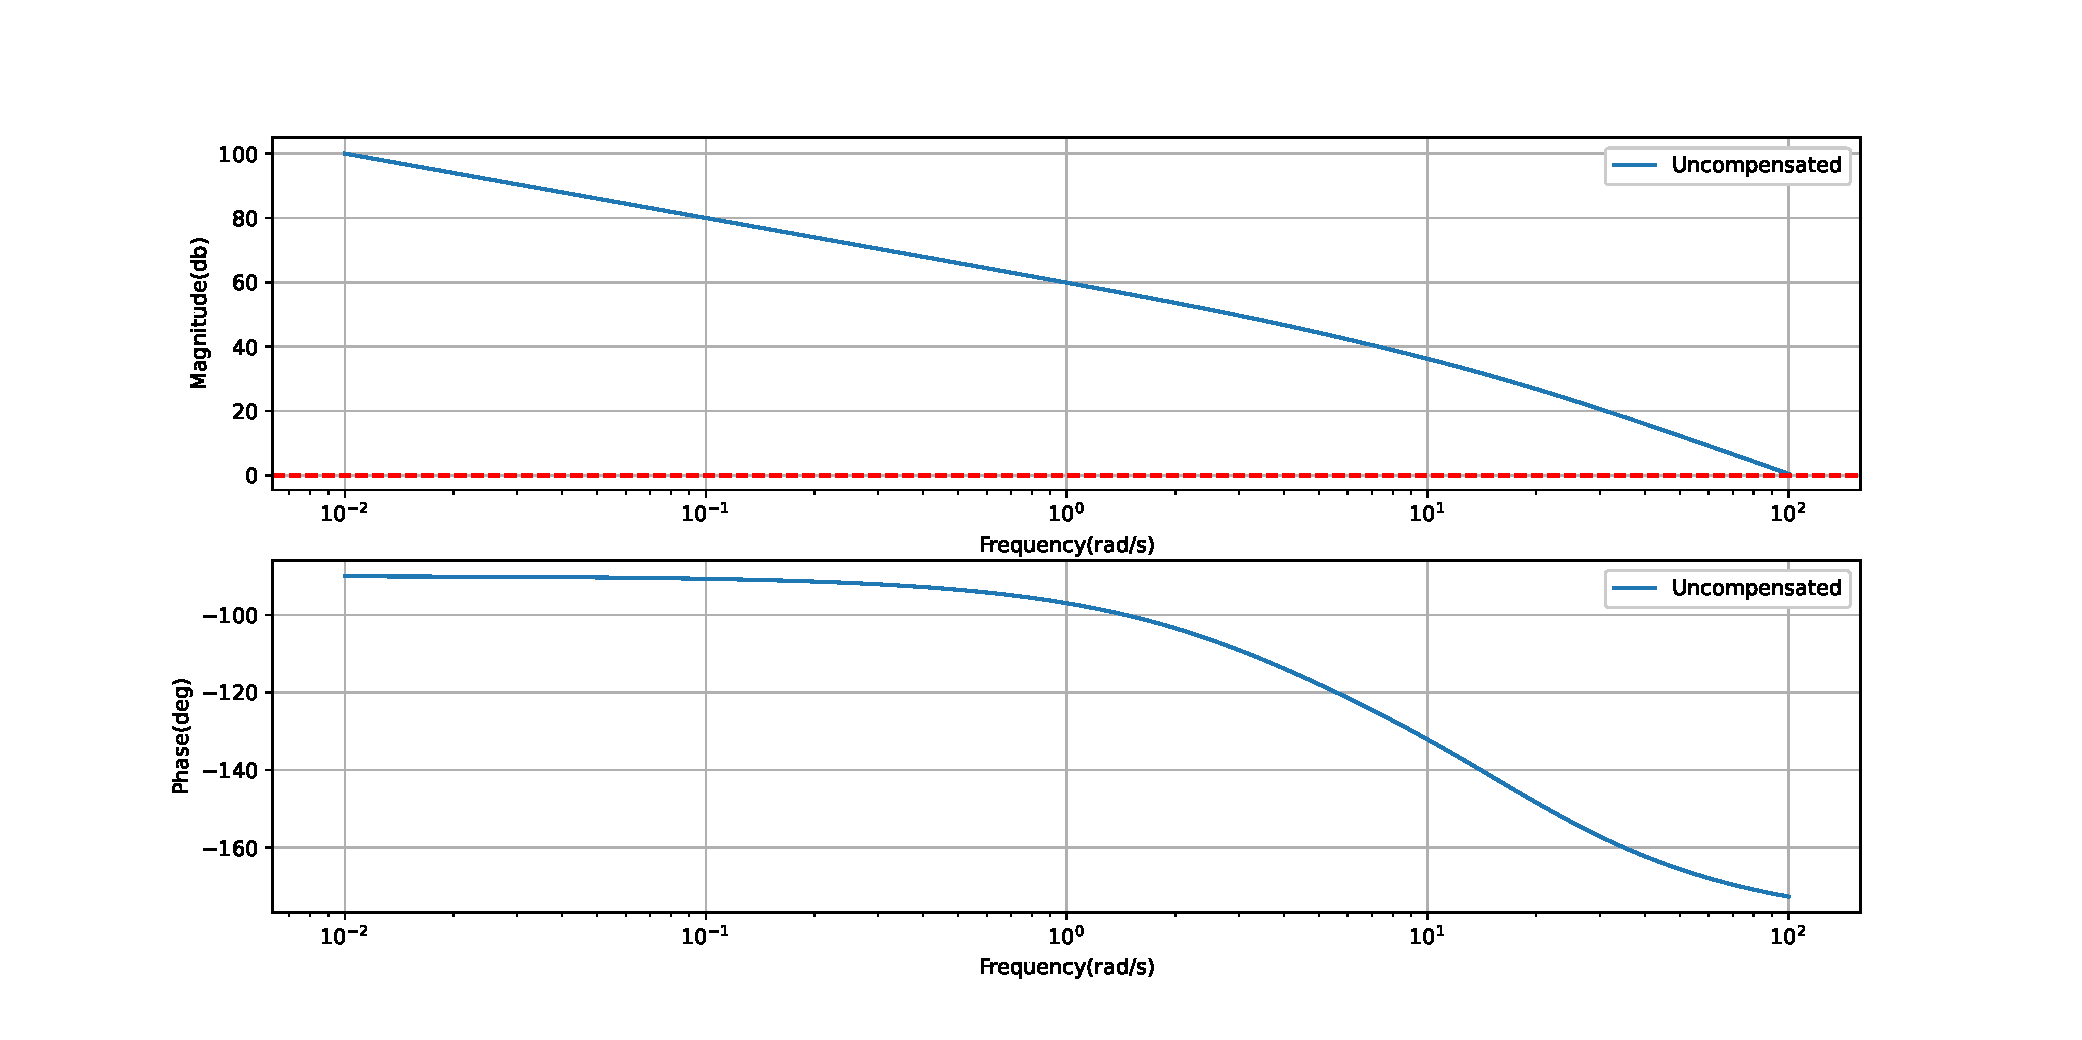
\includegraphics[width=\columnwidth]{./figs/ee18btech11012/ee18btech11012.eps}
\caption{}
\label{fig:ee18btech11012_2}
\end{figure}
%%
The following code verifies the result.
\begin{lstlisting}
codes/ee18btech11012/ee18btech11012_1.py
\end{lstlisting}
Relation between \%OS and Damping ratio
\begin{align}
\zeta &= \frac{-\ln(\%OS/100)}{\sqrt{(\pi)^2 + (\ln(\%OS/100))^2}}
\end{align}
\begin{align}
\implies\zeta &= 0.517 
\end{align}
Phase Margin for a Damping ratio is given by
\begin{align}
\phi_{m} &= 90\degree - \arctan(\frac{\sqrt{-2\zeta^2+\sqrt{1+4\zeta^4}}}{2\zeta}
\end{align}
\begin{align}
\implies \phi_{m} &= 53.17\degree
\end{align}
For an additional 5\degree for lag compensation,Phase margin is
\begin{align}
    \phi_{m} &= 53.17\degree + 5\degree= 58.17\degree
\end{align}
\textbf{Note} : Adding 5\degree phase angle to compensate the phase angle contribution of the lag compensator.
Bandwidth frequency is given by
\begin{align}
\omega_{BW} &= \omega_{n}(\sqrt{(1-2\zeta^2)+\sqrt{4\zeta^4-4\zeta^2+2}})
\end{align}
where
\begin{align}
    \omega_{n} &= \frac{4}{T_{s}\zeta}
\end{align}
Given settling time = 0.1 sec then 
\begin{align}
    \omega_{n} &= 77.37 rad/sec 
\end{align}
then
\begin{align}
    \omega_{BW} &= 96.91 rad/sec
\end{align}
\item Designing Lag-Lead Compensator Gc(s) \\
\solution 
General lag-lead compensator 
\begin{align}
G_{c}(s) &= \left(\frac{s+\frac{1}{T_1}}{s+\frac{\gamma}{T_1}}\right)\left(\frac{s+\frac{1}{T_2}}{s+\frac{1}{\gamma T_2}}\right) 
\end{align}
\begin{itemize}
\item Choose the new phase-margin frequency 
\begin{align}
    \omega_{Pm} &= 0.8 \omega_{BW} &= 77.53 rad/sec
\end{align}
\item At this phase-margin frequency,Phase angle is -170.52\degree.
\item Then the conribution required from the lead is
\begin{align}
    \phi_{max} &= 58.17-(180-170.52)=48.69\degree.
\end{align}

\item Now Using the relation 
\begin{align}
    \phi_{max} &= \sin^{-1}(\frac{1-\beta}{1+\beta})
\end{align}
then we get
\begin{align}
    \beta &= 0.142
\end{align}
\item \underline{Lag Compensator Design}:The Compensator must have a dc gain of unity to retain the value of Kv that we have already designed by setting K = 10714.
\begin{align}
    z_{clag} &= \frac{\omega_{Pm}}{10}=\frac{77.53}{10}=7.753
\end{align}
\begin{align}
    p_{clag} &= z_{clag}*\beta=1.102
\end{align}
Gain in the lag compensator is 
\begin{align}
    K_{clag} &= \frac{p_{clag}}{z_{clag}}=0.1421
\end{align}
\item Hence the lag compensator transfer function is
\begin{align}
 G_{clag}(s) &= \frac{0.1421(s+7.753)}{s+1.102} 
\end{align}
\item \underline{Lead Compensator Design}:DC gain for this must be unity.

\textbf{Relations to find T and $\beta$}:
The Compensator's magnitude at the phase margin frequency $\omega_{max}$
\begin{align}
     |G_{c}(j\omega_{max})| &= \frac{1}{\sqrt{\beta}} 
\end{align}
\begin{align}
    T &= \frac{1}{\omega_{max}\sqrt{\beta}}
\end{align}
So,To find transfer function
\begin{align}
    z_{lead} &= \frac{1}{T_{2}}=\omega_{Pm}*\sqrt{\beta}=29.92
\end{align}
\begin{align}
    p_{lead} &= \frac{z_{lead}}{\beta}=205.74,K_{lead}=\frac{p_{lead}}{z_{lead}}=7.04
\end{align}
\item Thus lead compensator transfer function is 
\begin{align}
    G_{lead} &= \frac{7.04(s+29.22)}{s+205.74} 
\end{align}
\item So the overall compensator tranfer function is
\begin{align}
    G_{c}(s) &= G_{clag}(s)G_{lead}(s)
\end{align}
\begin{align}
G_{c}(s)&=\frac{1.000384(s+7.753)(s+29.23)}{(s+1.102)(s+205.7)}
\end{align}
\end{itemize}
\item Verifying Lag-lead Compensator using Plots \\
\solution 
Magnitude and Phase plot
\begin{figure}[!ht]
\centering
  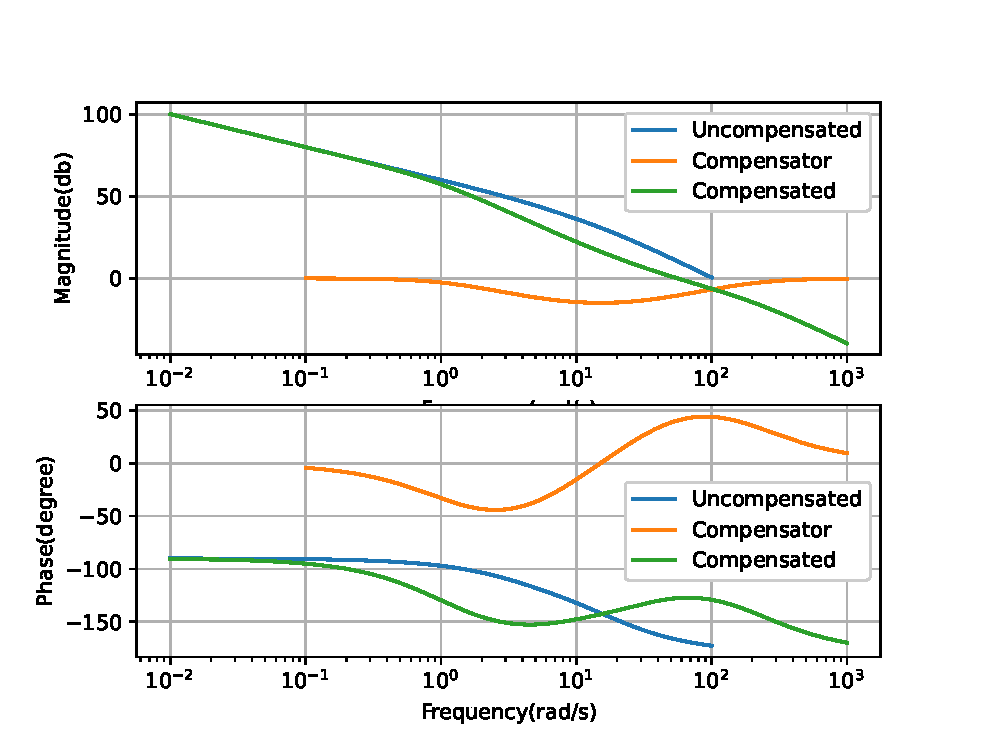
\includegraphics[width=\columnwidth]{./figs/ee18btech11012/ee18btech11012_2.eps}
\caption{}
\label{fig:ee18btech11012_3}
\end{figure}
The following code 
\begin{lstlisting}
codes/ee18btech11012/ee18btech11012_2.py
\end{lstlisting}
\item Verifying in time domain \\
\solution 
Time response for a unit step function
\begin{figure}[!ht]
\centering
  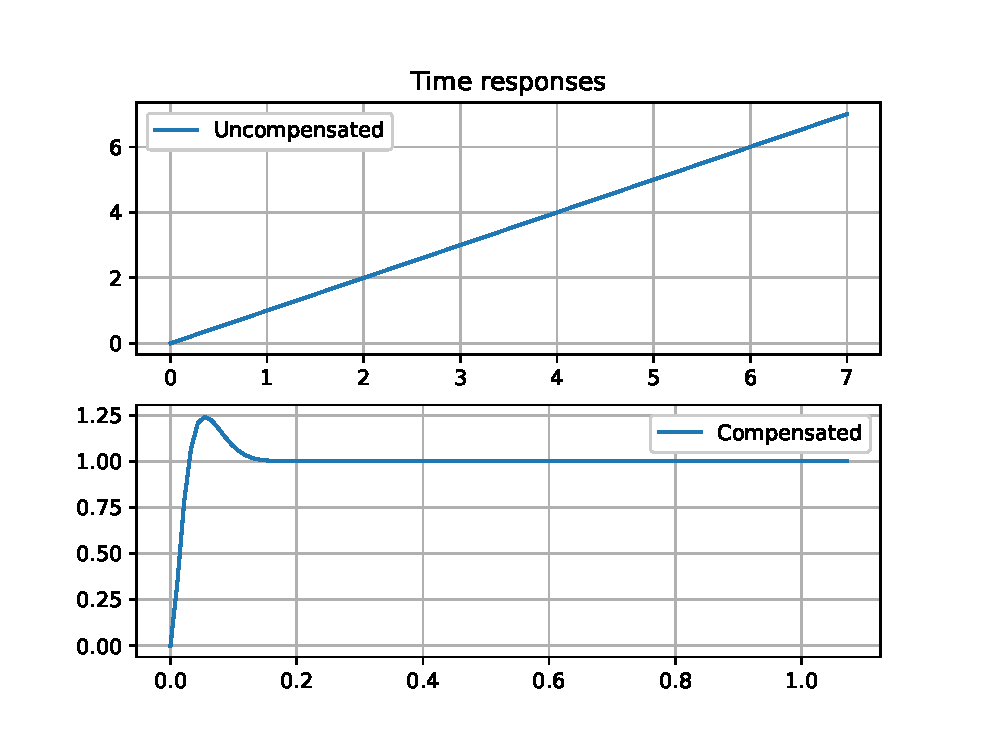
\includegraphics[width=\columnwidth]{./figs/ee18btech11012/ee18btech11012_3.eps}
\caption{}
\label{fig:ee18btech11012_4} 
\end{figure}
The following code can be verified
\begin{lstlisting}
codes/ee18btech11012/ee18btech11012_3.py
\end{lstlisting}
\item Verifying the designed lag-lead compensator \\
\solution 
\begin{table}[!ht]
\centering
\input{./tables/ee18btech11012/ee18btech11012_table1.tex}
\caption{Comparing the desired and obtained results}
\label{table:ee18btech11012_table1}
\end{table}
\end{enumerate}
}
\end{center}
\caption{}
\label{fig:ee18btech11012_1;}
\end{figure}
%
Velocity error constant  
\begin{align}
K_{v} &=  \lim_{s \to 0}sG(s)
\end{align}
\begin{align}
\lim_{s \to 0}s\frac{K(s+7)}{s(s+5)(s+15)} &= 1000
\end{align}
\begin{align}
\implies K &= 10714
\end{align}
Bode plot of G(s) for the value of K
%%
\begin{figure}[!ht]
\centering
  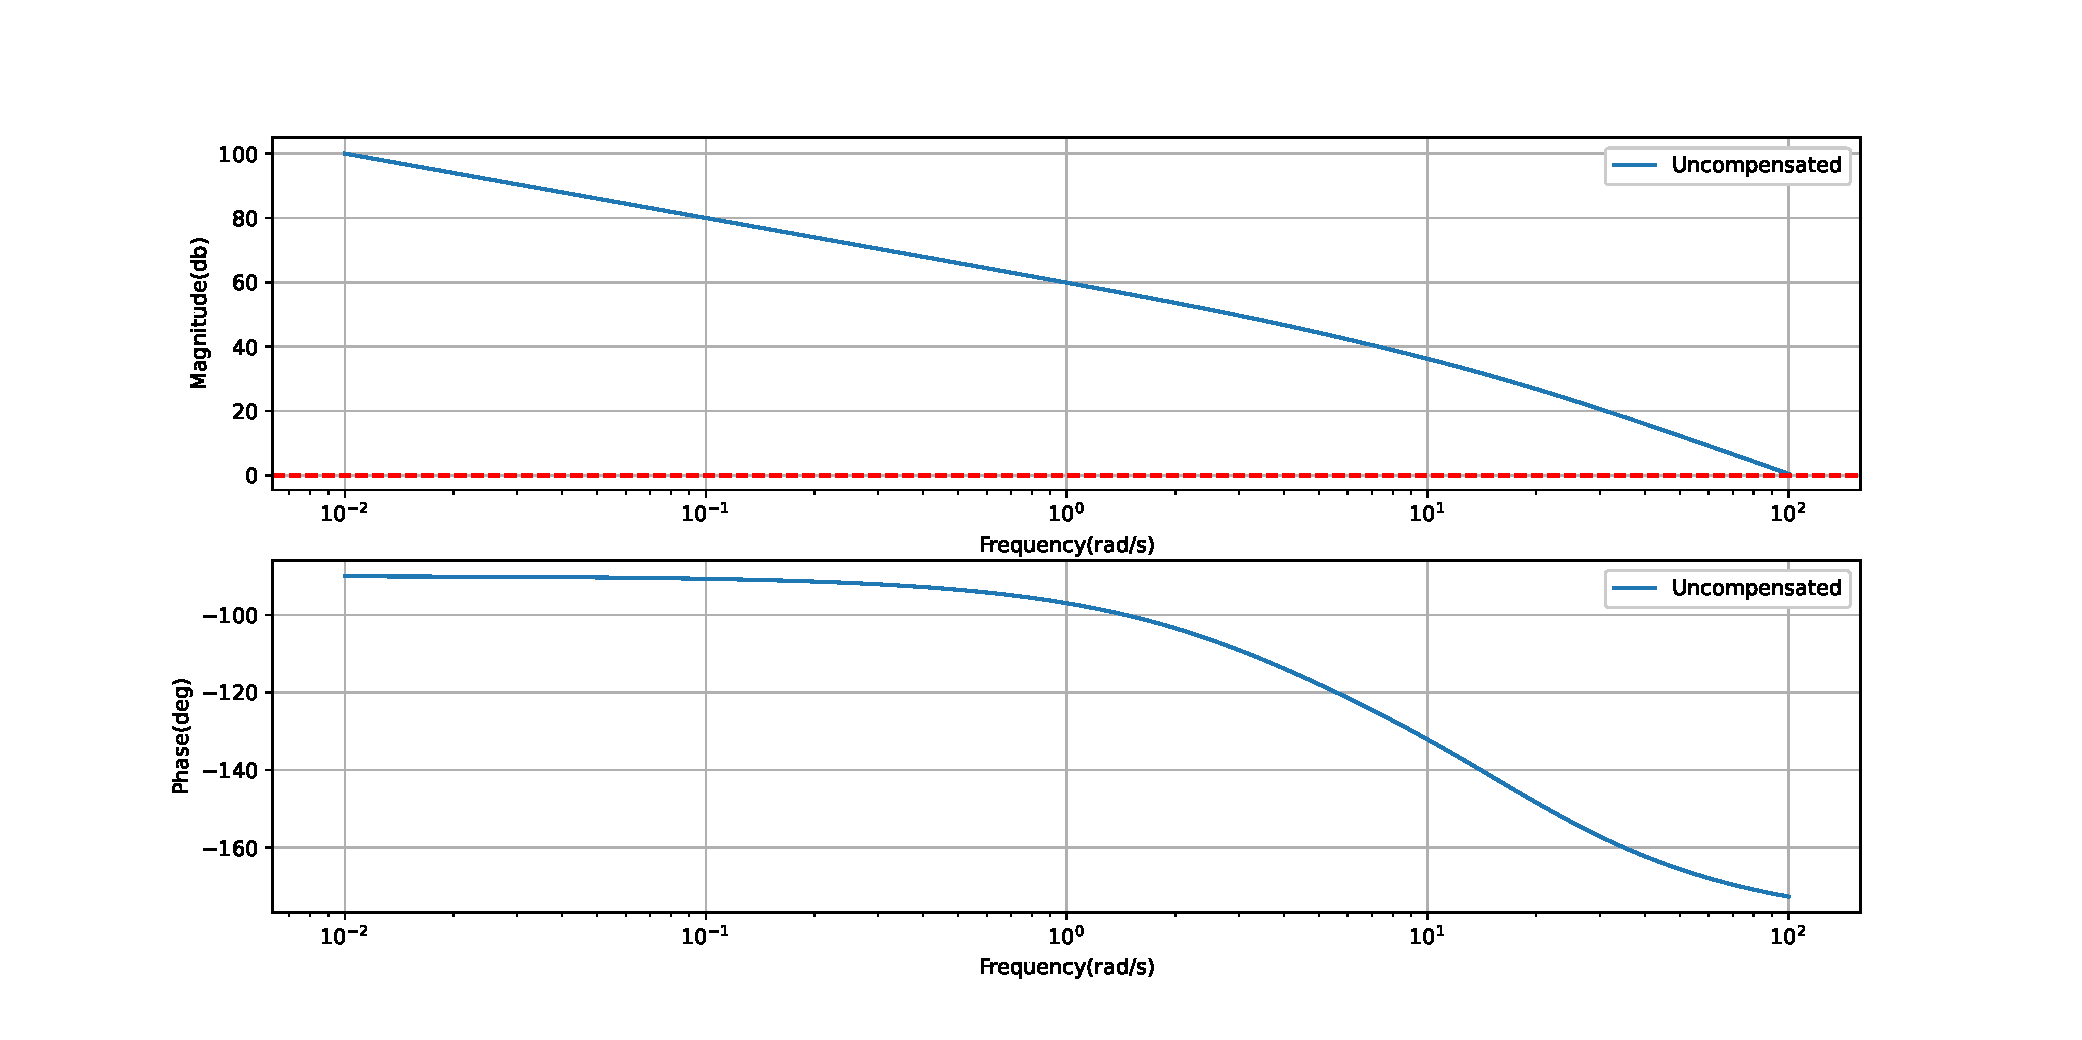
\includegraphics[width=\columnwidth]{./figs/ee18btech11012/ee18btech11012.eps}
\caption{}
\label{fig:ee18btech11012_2}
\end{figure}
%%
The following code verifies the result.
\begin{lstlisting}
codes/ee18btech11012/ee18btech11012_1.py
\end{lstlisting}
Relation between \%OS and Damping ratio
\begin{align}
\zeta &= \frac{-\ln(\%OS/100)}{\sqrt{(\pi)^2 + (\ln(\%OS/100))^2}}
\end{align}
\begin{align}
\implies\zeta &= 0.517 
\end{align}
Phase Margin for a Damping ratio is given by
\begin{align}
\phi_{m} &= 90\degree - \arctan(\frac{\sqrt{-2\zeta^2+\sqrt{1+4\zeta^4}}}{2\zeta}
\end{align}
\begin{align}
\implies \phi_{m} &= 53.17\degree
\end{align}
For an additional 5\degree for lag compensation,Phase margin is
\begin{align}
    \phi_{m} &= 53.17\degree + 5\degree= 58.17\degree
\end{align}
\textbf{Note} : Adding 5\degree phase angle to compensate the phase angle contribution of the lag compensator.
Bandwidth frequency is given by
\begin{align}
\omega_{BW} &= \omega_{n}(\sqrt{(1-2\zeta^2)+\sqrt{4\zeta^4-4\zeta^2+2}})
\end{align}
where
\begin{align}
    \omega_{n} &= \frac{4}{T_{s}\zeta}
\end{align}
Given settling time = 0.1 sec then 
\begin{align}
    \omega_{n} &= 77.37 rad/sec 
\end{align}
then
\begin{align}
    \omega_{BW} &= 96.91 rad/sec
\end{align}
\item Designing Lag-Lead Compensator Gc(s) \\
\solution 
General lag-lead compensator 
\begin{align}
G_{c}(s) &= \left(\frac{s+\frac{1}{T_1}}{s+\frac{\gamma}{T_1}}\right)\left(\frac{s+\frac{1}{T_2}}{s+\frac{1}{\gamma T_2}}\right) 
\end{align}
\begin{itemize}
\item Choose the new phase-margin frequency 
\begin{align}
    \omega_{Pm} &= 0.8 \omega_{BW} &= 77.53 rad/sec
\end{align}
\item At this phase-margin frequency,Phase angle is -170.52\degree.
\item Then the conribution required from the lead is
\begin{align}
    \phi_{max} &= 58.17-(180-170.52)=48.69\degree.
\end{align}

\item Now Using the relation 
\begin{align}
    \phi_{max} &= \sin^{-1}(\frac{1-\beta}{1+\beta})
\end{align}
then we get
\begin{align}
    \beta &= 0.142
\end{align}
\item \underline{Lag Compensator Design}:The Compensator must have a dc gain of unity to retain the value of Kv that we have already designed by setting K = 10714.
\begin{align}
    z_{clag} &= \frac{\omega_{Pm}}{10}=\frac{77.53}{10}=7.753
\end{align}
\begin{align}
    p_{clag} &= z_{clag}*\beta=1.102
\end{align}
Gain in the lag compensator is 
\begin{align}
    K_{clag} &= \frac{p_{clag}}{z_{clag}}=0.1421
\end{align}
\item Hence the lag compensator transfer function is
\begin{align}
 G_{clag}(s) &= \frac{0.1421(s+7.753)}{s+1.102} 
\end{align}
\item \underline{Lead Compensator Design}:DC gain for this must be unity.

\textbf{Relations to find T and $\beta$}:
The Compensator's magnitude at the phase margin frequency $\omega_{max}$
\begin{align}
     |G_{c}(j\omega_{max})| &= \frac{1}{\sqrt{\beta}} 
\end{align}
\begin{align}
    T &= \frac{1}{\omega_{max}\sqrt{\beta}}
\end{align}
So,To find transfer function
\begin{align}
    z_{lead} &= \frac{1}{T_{2}}=\omega_{Pm}*\sqrt{\beta}=29.92
\end{align}
\begin{align}
    p_{lead} &= \frac{z_{lead}}{\beta}=205.74,K_{lead}=\frac{p_{lead}}{z_{lead}}=7.04
\end{align}
\item Thus lead compensator transfer function is 
\begin{align}
    G_{lead} &= \frac{7.04(s+29.22)}{s+205.74} 
\end{align}
\item So the overall compensator tranfer function is
\begin{align}
    G_{c}(s) &= G_{clag}(s)G_{lead}(s)
\end{align}
\begin{align}
G_{c}(s)&=\frac{1.000384(s+7.753)(s+29.23)}{(s+1.102)(s+205.7)}
\end{align}
\end{itemize}
\item Verifying Lag-lead Compensator using Plots \\
\solution 
Magnitude and Phase plot
\begin{figure}[!ht]
\centering
  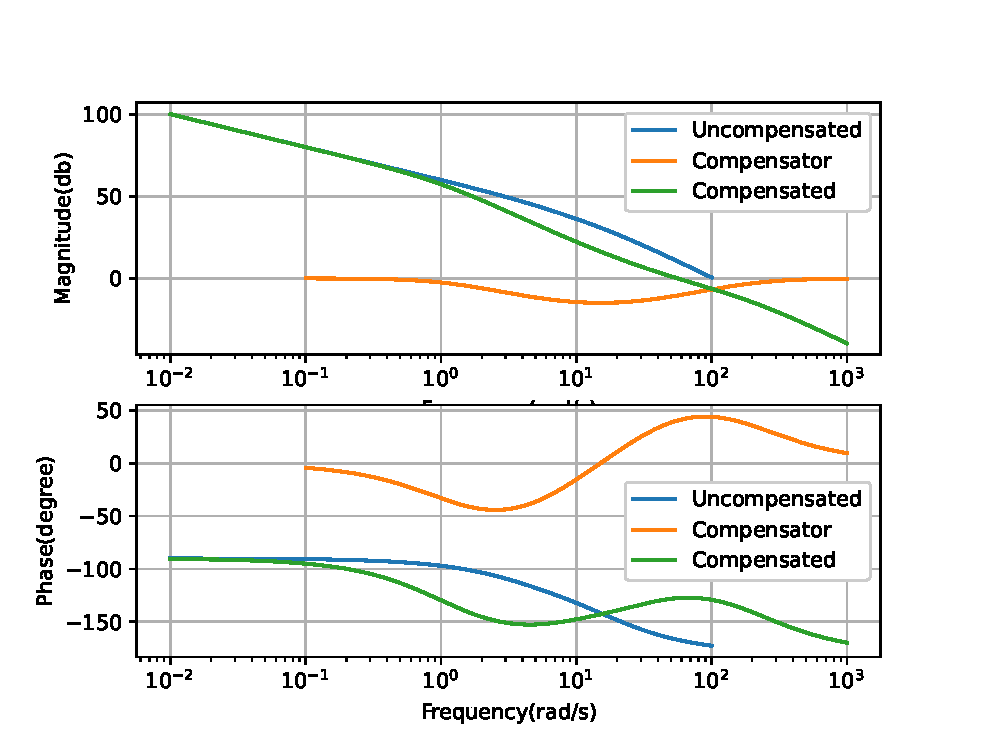
\includegraphics[width=\columnwidth]{./figs/ee18btech11012/ee18btech11012_2.eps}
\caption{}
\label{fig:ee18btech11012_3}
\end{figure}
The following code 
\begin{lstlisting}
codes/ee18btech11012/ee18btech11012_2.py
\end{lstlisting}
\item Verifying in time domain \\
\solution 
Time response for a unit step function
\begin{figure}[!ht]
\centering
  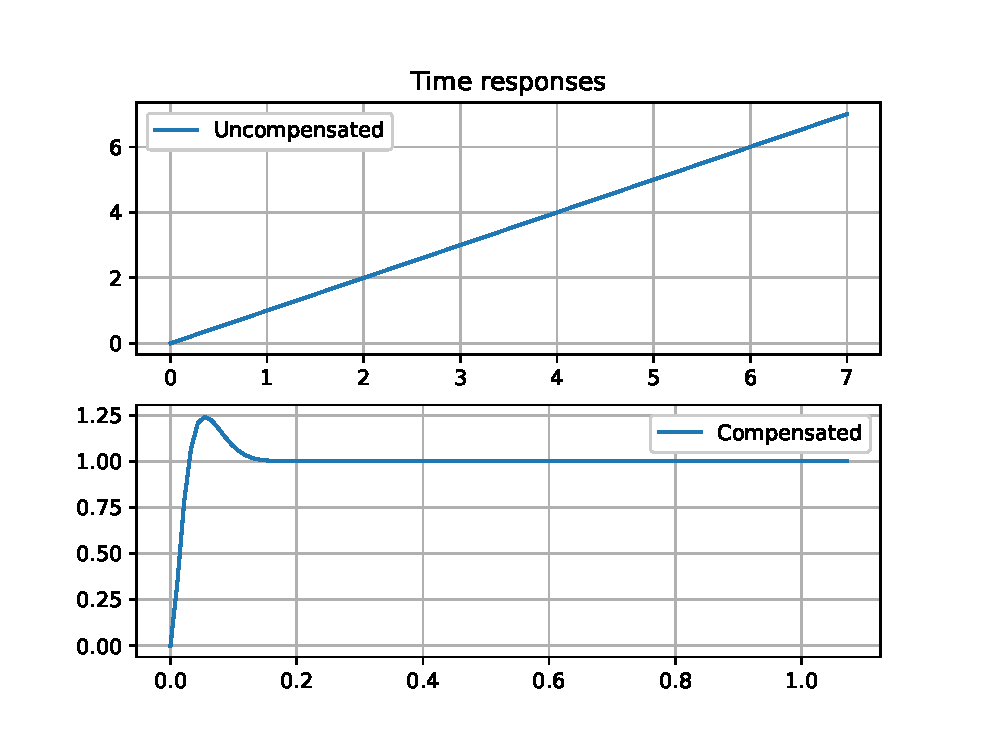
\includegraphics[width=\columnwidth]{./figs/ee18btech11012/ee18btech11012_3.eps}
\caption{}
\label{fig:ee18btech11012_4} 
\end{figure}
The following code can be verified
\begin{lstlisting}
codes/ee18btech11012/ee18btech11012_3.py
\end{lstlisting}
\item Verifying the designed lag-lead compensator \\
\solution 
\begin{table}[!ht]
\centering
%%%%%%%%%%%%%%%%%%%%%%%%%%%%%%%%%%%%%%%%%%%%%%%%%%%%%%%%%%%%%%%%%%%%%%
%%                                                                  %%
%%  This is the header of a LaTeX2e file exported from Gnumeric.    %%
%%                                                                  %%
%%  This file can be compiled as it stands or included in another   %%
%%  LaTeX document. The table is based on the longtable package so  %%
%%  the longtable options (headers, footers...) can be set in the   %%
%%  preamble section below (see PRAMBLE).                           %%
%%                                                                  %%
%%  To include the file in another, the following two lines must be %%
%%  in the including file:                                          %%
%%        \def\inputGnumericTable{}                                 %%
%%  at the beginning of the file and:                               %%
%%        \input{name-of-this-file.tex}                             %%
%%  where the table is to be placed. Note also that the including   %%
%%  file must use the following packages for the table to be        %%
%%  rendered correctly:                                             %%
%%    \usepackage[latin1]{inputenc}                                 %%
%%    \usepackage{color}                                            %%
%%    \usepackage{array}                                            %%
%%    \usepackage{longtable}                                        %%
%%    \usepackage{calc}                                             %%
%%    \usepackage{multirow}                                         %%
%%    \usepackage{hhline}                                           %%
%%    \usepackage{ifthen}                                           %%
%%  optionally (for landscape tables embedded in another document): %%
%%    \usepackage{lscape}                                           %%
%%                                                                  %%
%%%%%%%%%%%%%%%%%%%%%%%%%%%%%%%%%%%%%%%%%%%%%%%%%%%%%%%%%%%%%%%%%%%%%%



%%  This section checks if we are begin input into another file or  %%
%%  the file will be compiled alone. First use a macro taken from   %%
%%  the TeXbook ex 7.7 (suggestion of Han-Wen Nienhuys).            %%
\def\ifundefined#1{\expandafter\ifx\csname#1\endcsname\relax}


%%  Check for the \def token for inputed files. If it is not        %%
%%  defined, the file will be processed as a standalone and the     %%
%%  preamble will be used.                                          %%
\ifundefined{inputGnumericTable}

%%  We must be able to close or not the document at the end.        %%
	\def\gnumericTableEnd{\end{document}}


%%%%%%%%%%%%%%%%%%%%%%%%%%%%%%%%%%%%%%%%%%%%%%%%%%%%%%%%%%%%%%%%%%%%%%
%%                                                                  %%
%%  This is the PREAMBLE. Change these values to get the right      %%
%%  paper size and other niceties.                                  %%
%%                                                                  %%
%%%%%%%%%%%%%%%%%%%%%%%%%%%%%%%%%%%%%%%%%%%%%%%%%%%%%%%%%%%%%%%%%%%%%%

	\documentclass[12pt%
			  %,landscape%
                    ]{report}
       \usepackage[latin1]{inputenc}
       \usepackage{fullpage}
       \usepackage{color}
       \usepackage{array}
       \usepackage{longtable}
       \usepackage{calc}
       \usepackage{multirow}
       \usepackage{hhline}
       \usepackage{ifthen}



%%  End of the preamble for the standalone. The next section is for %%
%%  documents which are included into other LaTeX2e files.          %%
\else

%%  We are not a stand alone document. For a regular table, we will %%
%%  have no preamble and only define the closing to mean nothing.   %%
    \def\gnumericTableEnd{}

%%  If we want landscape mode in an embedded document, comment out  %%
%%  the line above and uncomment the two below. The table will      %%
%%  begin on a new page and run in landscape mode.                  %%
%       \def\gnumericTableEnd{\end{landscape}}
%       \begin{landscape}


%%  End of the else clause for this file being \input.              %%
\fi

%%%%%%%%%%%%%%%%%%%%%%%%%%%%%%%%%%%%%%%%%%%%%%%%%%%%%%%%%%%%%%%%%%%%%%
%%                                                                  %%
%%  The rest is the gnumeric table, except for the closing          %%
%%  statement. Changes below will alter the table's appearance.     %%
%%                                                                  %%
%%%%%%%%%%%%%%%%%%%%%%%%%%%%%%%%%%%%%%%%%%%%%%%%%%%%%%%%%%%%%%%%%%%%%%

\providecommand{\gnumericmathit}[1]{#1} 
%%  Uncomment the next line if you would like your numbers to be in %%
%%  italics if they are italizised in the gnumeric table.           %%
%\renewcommand{\gnumericmathit}[1]{\mathit{#1}}
\providecommand{\gnumericPB}[1]%
{\let\gnumericTemp=\\#1\let\\=\gnumericTemp\hspace{0pt}}
 \ifundefined{gnumericTableWidthDefined}
        \newlength{\gnumericTableWidth}
        \newlength{\gnumericTableWidthComplete}
        \newlength{\gnumericMultiRowLength}
        \global\def\gnumericTableWidthDefined{}
 \fi
%% The following setting protects this code from babel shorthands.  %%
 \ifthenelse{\isundefined{\languageshorthands}}{}{\languageshorthands{english}}
%%  The default table format retains the relative column widths of  %%
%%  gnumeric. They can easily be changed to c, r or l. In that case %%
%%  you may want to comment out the next line and uncomment the one %%
%%  thereafter                                                      %%
\providecommand\gnumbox{\makebox[0pt]}
%%\providecommand\gnumbox[1][]{\makebox}

%% to adjust positions in multirow situations                       %%
\setlength{\bigstrutjot}{\jot}
\setlength{\extrarowheight}{\doublerulesep}

%%  The \setlongtables command keeps column widths the same across  %%
%%  pages. Simply comment out next line for varying column widths.  %%
\setlongtables

\setlength\gnumericTableWidth{%
	70pt+%
	70pt+%
	70pt+%
0pt}
\def\gumericNumCols{3}
\setlength\gnumericTableWidthComplete{\gnumericTableWidth+%
         \tabcolsep*\gumericNumCols*2+\arrayrulewidth*\gumericNumCols}
\ifthenelse{\lengthtest{\gnumericTableWidthComplete > \linewidth}}%
         {\def\gnumericScale{\ratio{\linewidth-%
                        \tabcolsep*\gumericNumCols*2-%
                        \arrayrulewidth*\gumericNumCols}%
{\gnumericTableWidth}}}%
{\def\gnumericScale{1}}

%%%%%%%%%%%%%%%%%%%%%%%%%%%%%%%%%%%%%%%%%%%%%%%%%%%%%%%%%%%%%%%%%%%%%%
%%                                                                  %%
%% The following are the widths of the various columns. We are      %%
%% defining them here because then they are easier to change.       %%
%% Depending on the cell formats we may use them more than once.    %%
%%                                                                  %%
%%%%%%%%%%%%%%%%%%%%%%%%%%%%%%%%%%%%%%%%%%%%%%%%%%%%%%%%%%%%%%%%%%%%%%

\ifthenelse{\isundefined{\gnumericColA}}{\newlength{\gnumericColA}}{}\settowidth{\gnumericColA}{\begin{tabular}{@{}p{70pt*\gnumericScale}@{}}x\end{tabular}}
\ifthenelse{\isundefined{\gnumericColB}}{\newlength{\gnumericColB}}{}\settowidth{\gnumericColB}{\begin{tabular}{@{}p{70pt*\gnumericScale}@{}}x\end{tabular}}
\ifthenelse{\isundefined{\gnumericColC}}{\newlength{\gnumericColC}}{}\settowidth{\gnumericColC}{\begin{tabular}{@{}p{70pt*\gnumericScale}@{}}x\end{tabular}}

\begin{tabular}[c]{%
	b{\gnumericColA}%
	b{\gnumericColB}%
	b{\gnumericColC}%
	}

%%%%%%%%%%%%%%%%%%%%%%%%%%%%%%%%%%%%%%%%%%%%%%%%%%%%%%%%%%%%%%%%%%%%%%
%%  The longtable options. (Caption, headers... see Goosens, p.124) %%
%	\caption{The Table Caption.}             \\	%
% \hline	% Across the top of the table.
%%  The rest of these options are table rows which are placed on    %%
%%  the first, last or every page. Use \multicolumn if you want.    %%

%%  Header for the first page.                                      %%
%	\multicolumn{3}{c}{The First Header} \\ \hline 
%	\multicolumn{1}{c}{colTag}	%Column 1
%	&\multicolumn{1}{c}{colTag}	%Column 2
%	&\multicolumn{1}{c}{colTag}	\\ \hline %Last column
%	\endfirsthead

%%  The running header definition.                                  %%
%	\hline
%	\multicolumn{3}{l}{\ldots\small\slshape continued} \\ \hline
%	\multicolumn{1}{c}{colTag}	%Column 1
%	&\multicolumn{1}{c}{colTag}	%Column 2
%	&\multicolumn{1}{c}{colTag}	\\ \hline %Last column
%	\endhead

%%  The running footer definition.                                  %%
%	\hline
%	\multicolumn{3}{r}{\small\slshape continued\ldots} \\
%	\endfoot

%%  The ending footer definition.                                   %%
%	\multicolumn{3}{c}{That's all folks} \\ \hline 
%	\endlastfoot
%%%%%%%%%%%%%%%%%%%%%%%%%%%%%%%%%%%%%%%%%%%%%%%%%%%%%%%%%%%%%%%%%%%%%%

\hhline{|-|-|-|}
	 \multicolumn{1}{|p{\gnumericColA}|}%
	{\gnumericPB{\centering}\textbf{Parameter Specification}}
	&\multicolumn{1}{p{\gnumericColB}|}%
	{\gnumericPB{\centering}\textbf{Proposed}}
	&\multicolumn{1}{p{\gnumericColC}|}%
	{\gnumericPB{\centering}\textbf{Actual}}

\\
\hhline{|-|-|-|}
	 \multicolumn{1}{|p{\gnumericColA}|}%
	{\gnumericPB{\centering}Phase Margin}
	&\multicolumn{1}{p{\gnumericColB}|}%
	{\gnumericPB{\centering}53.17\degree}
	&\multicolumn{1}{p{\gnumericColC}|}%
	{\gnumericPB{\centering}53.3994\degree}
	
\\
\hhline{|-|-|-|}
	 \multicolumn{1}{|p{\gnumericColA}|}%
	{\gnumericPB{\centering}$K_{v}$}
	&\multicolumn{1}{p{\gnumericColB}|}%
	{\gnumericPB{\centering}1000}
	&\multicolumn{1}{p{\gnumericColC}|}%
	{\gnumericPB{\centering}1023.67}
\\
\hhline{|-|-|-|}
	 \multicolumn{1}{|p{\gnumericColA}|}%
	{\gnumericPB{\centering}Phase Margin frequency}
	&\multicolumn{1}{p{\gnumericColB}|}%
	{\gnumericPB{\centering}77.53}
	&\multicolumn{1}{p{\gnumericColC}|}%
	{\gnumericPB{\centering}55.5874}
	
\\

\hhline{|-|-|-|}
\end{tabular}

\ifthenelse{\isundefined{\languageshorthands}}{}{\languageshorthands{\languagename}}
\gnumericTableEnd

\caption{Comparing the desired and obtained results}
\label{table:ee18btech11012_table1}
\end{table}
\end{enumerate}
}
\end{center}
\caption{}
\label{fig:ee18btech11012_1;}
\end{figure}
%
Velocity error constant  
\begin{align}
K_{v} &=  \lim_{s \to 0}sG(s)
\end{align}
\begin{align}
\lim_{s \to 0}s\frac{K(s+7)}{s(s+5)(s+15)} &= 1000
\end{align}
\begin{align}
\implies K &= 10714
\end{align}
Bode plot of G(s) for the value of K
%%
\begin{figure}[!ht]
\centering
  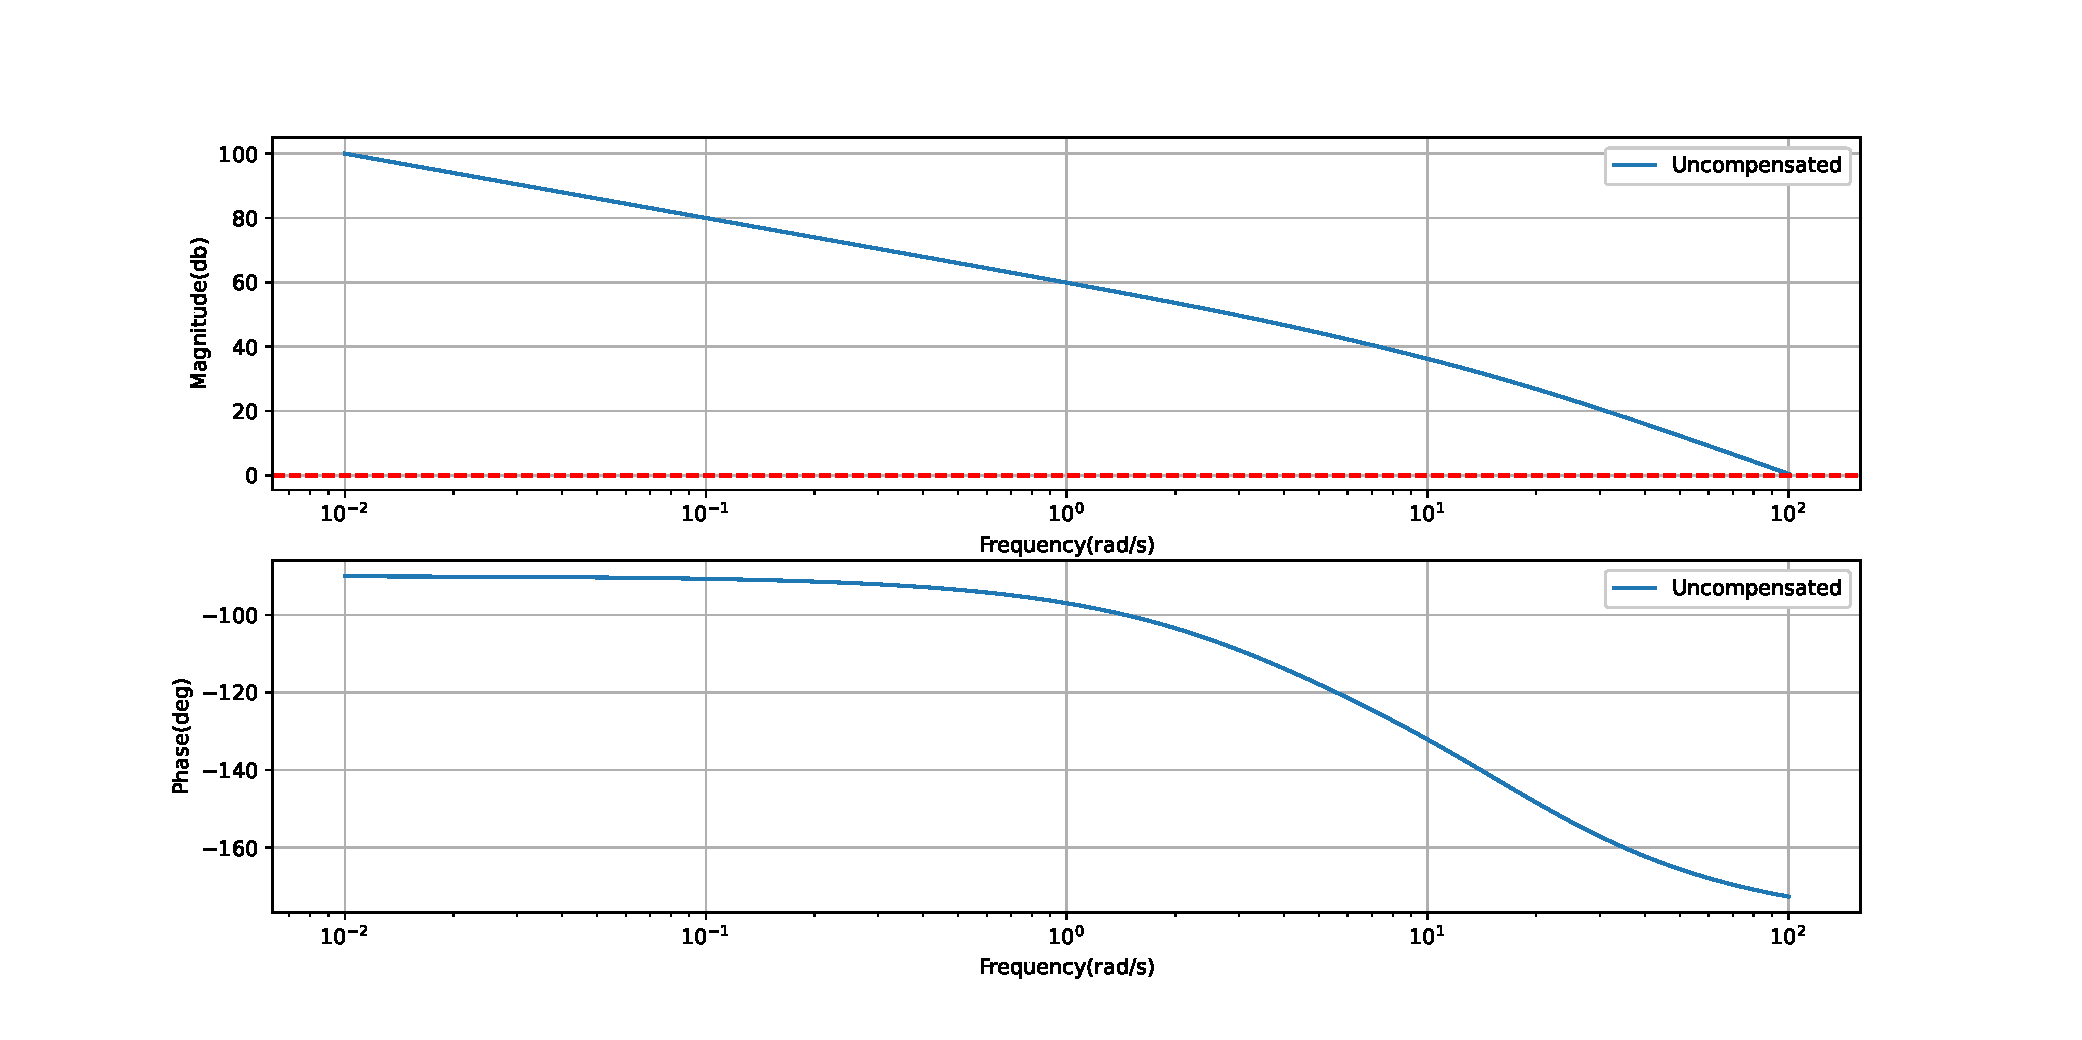
\includegraphics[width=\columnwidth]{./figs/ee18btech11012/ee18btech11012.eps}
\caption{}
\label{fig:ee18btech11012_2}
\end{figure}
%%
The following code verifies the result.
\begin{lstlisting}
codes/ee18btech11012/ee18btech11012_1.py
\end{lstlisting}
Relation between \%OS and Damping ratio
\begin{align}
\zeta &= \frac{-\ln(\%OS/100)}{\sqrt{(\pi)^2 + (\ln(\%OS/100))^2}}
\end{align}
\begin{align}
\implies\zeta &= 0.517 
\end{align}
Phase Margin for a Damping ratio is given by
\begin{align}
\phi_{m} &= 90\degree - \arctan(\frac{\sqrt{-2\zeta^2+\sqrt{1+4\zeta^4}}}{2\zeta}
\end{align}
\begin{align}
\implies \phi_{m} &= 53.17\degree
\end{align}
For an additional 5\degree for lag compensation,Phase margin is
\begin{align}
    \phi_{m} &= 53.17\degree + 5\degree= 58.17\degree
\end{align}
\textbf{Note} : Adding 5\degree phase angle to compensate the phase angle contribution of the lag compensator.
Bandwidth frequency is given by
\begin{align}
\omega_{BW} &= \omega_{n}(\sqrt{(1-2\zeta^2)+\sqrt{4\zeta^4-4\zeta^2+2}})
\end{align}
where
\begin{align}
    \omega_{n} &= \frac{4}{T_{s}\zeta}
\end{align}
Given settling time = 0.1 sec then 
\begin{align}
    \omega_{n} &= 77.37 rad/sec 
\end{align}
then
\begin{align}
    \omega_{BW} &= 96.91 rad/sec
\end{align}
\item Designing Lag-Lead Compensator Gc(s) \\
\solution 
General lag-lead compensator 
\begin{align}
G_{c}(s) &= \left(\frac{s+\frac{1}{T_1}}{s+\frac{\gamma}{T_1}}\right)\left(\frac{s+\frac{1}{T_2}}{s+\frac{1}{\gamma T_2}}\right) 
\end{align}
\begin{itemize}
\item Choose the new phase-margin frequency 
\begin{align}
    \omega_{Pm} &= 0.8 \omega_{BW} &= 77.53 rad/sec
\end{align}
\item At this phase-margin frequency,Phase angle is -170.52\degree.
\item Then the conribution required from the lead is
\begin{align}
    \phi_{max} &= 58.17-(180-170.52)=48.69\degree.
\end{align}

\item Now Using the relation 
\begin{align}
    \phi_{max} &= \sin^{-1}(\frac{1-\beta}{1+\beta})
\end{align}
then we get
\begin{align}
    \beta &= 0.142
\end{align}
\item \underline{Lag Compensator Design}:The Compensator must have a dc gain of unity to retain the value of Kv that we have already designed by setting K = 10714.
\begin{align}
    z_{clag} &= \frac{\omega_{Pm}}{10}=\frac{77.53}{10}=7.753
\end{align}
\begin{align}
    p_{clag} &= z_{clag}*\beta=1.102
\end{align}
Gain in the lag compensator is 
\begin{align}
    K_{clag} &= \frac{p_{clag}}{z_{clag}}=0.1421
\end{align}
\item Hence the lag compensator transfer function is
\begin{align}
 G_{clag}(s) &= \frac{0.1421(s+7.753)}{s+1.102} 
\end{align}
\item \underline{Lead Compensator Design}:DC gain for this must be unity.

\textbf{Relations to find T and $\beta$}:
The Compensator's magnitude at the phase margin frequency $\omega_{max}$
\begin{align}
     |G_{c}(j\omega_{max})| &= \frac{1}{\sqrt{\beta}} 
\end{align}
\begin{align}
    T &= \frac{1}{\omega_{max}\sqrt{\beta}}
\end{align}
So,To find transfer function
\begin{align}
    z_{lead} &= \frac{1}{T_{2}}=\omega_{Pm}*\sqrt{\beta}=29.92
\end{align}
\begin{align}
    p_{lead} &= \frac{z_{lead}}{\beta}=205.74,K_{lead}=\frac{p_{lead}}{z_{lead}}=7.04
\end{align}
\item Thus lead compensator transfer function is 
\begin{align}
    G_{lead} &= \frac{7.04(s+29.22)}{s+205.74} 
\end{align}
\item So the overall compensator tranfer function is
\begin{align}
    G_{c}(s) &= G_{clag}(s)G_{lead}(s)
\end{align}
\begin{align}
G_{c}(s)&=\frac{1.000384(s+7.753)(s+29.23)}{(s+1.102)(s+205.7)}
\end{align}
\end{itemize}
\item Verifying Lag-lead Compensator using Plots \\
\solution 
Magnitude and Phase plot
\begin{figure}[!ht]
\centering
  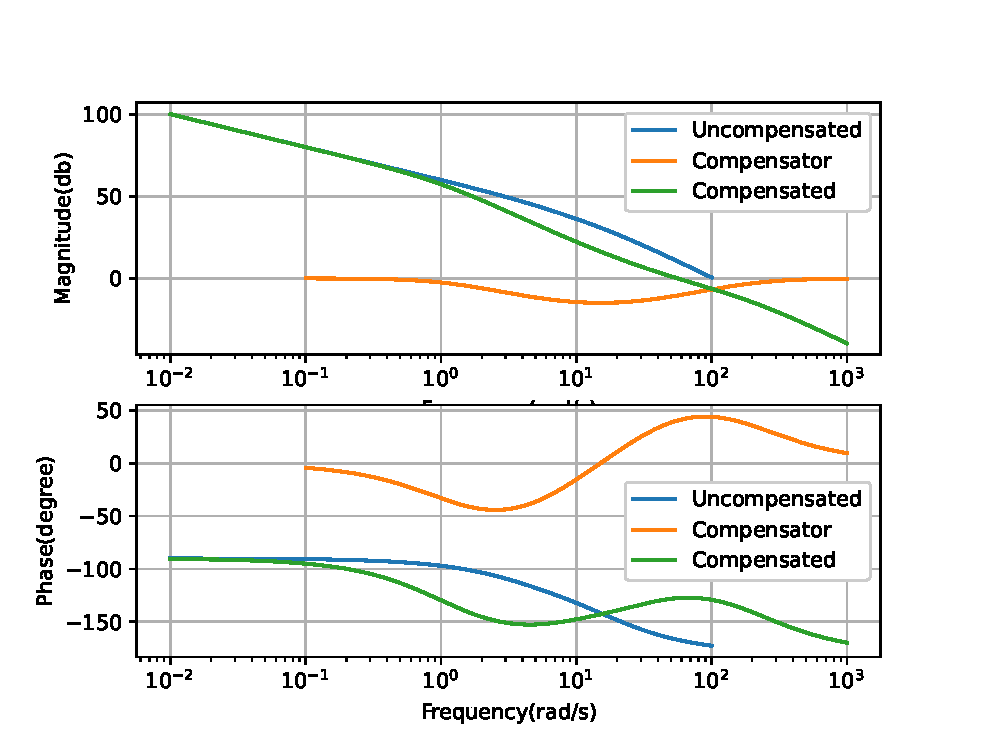
\includegraphics[width=\columnwidth]{./figs/ee18btech11012/ee18btech11012_2.eps}
\caption{}
\label{fig:ee18btech11012_3}
\end{figure}
The following code 
\begin{lstlisting}
codes/ee18btech11012/ee18btech11012_2.py
\end{lstlisting}
\item Verifying in time domain \\
\solution 
Time response for a unit step function
\begin{figure}[!ht]
\centering
  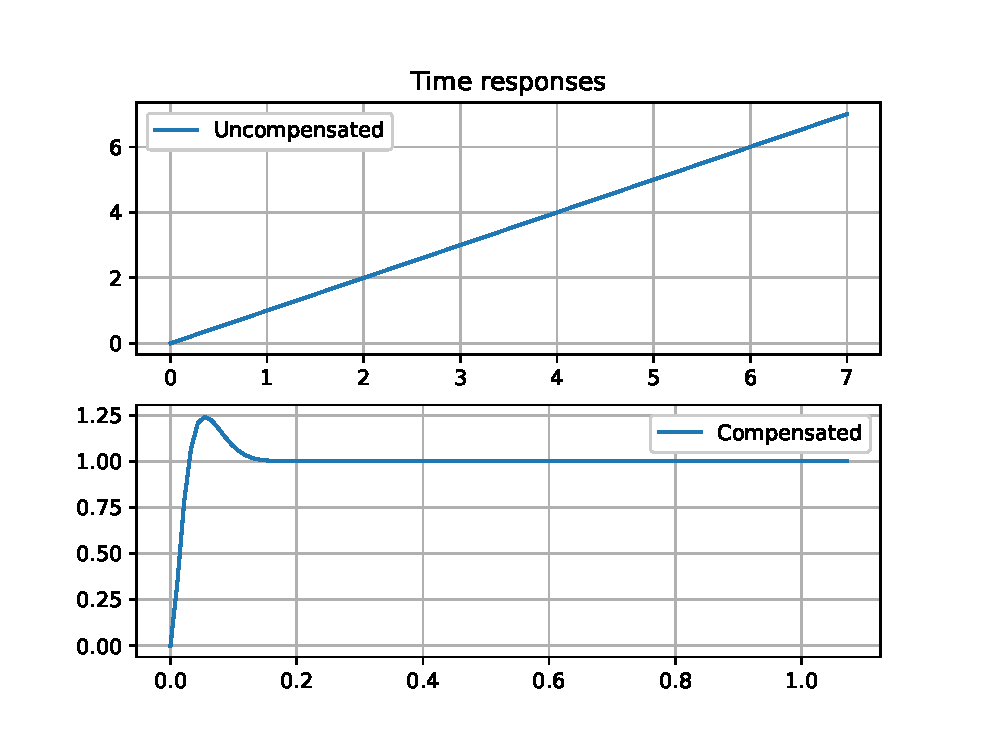
\includegraphics[width=\columnwidth]{./figs/ee18btech11012/ee18btech11012_3.eps}
\caption{}
\label{fig:ee18btech11012_4} 
\end{figure}
The following code can be verified
\begin{lstlisting}
codes/ee18btech11012/ee18btech11012_3.py
\end{lstlisting}
\item Verifying the designed lag-lead compensator \\
\solution 
\begin{table}[!ht]
\centering
%%%%%%%%%%%%%%%%%%%%%%%%%%%%%%%%%%%%%%%%%%%%%%%%%%%%%%%%%%%%%%%%%%%%%%
%%                                                                  %%
%%  This is the header of a LaTeX2e file exported from Gnumeric.    %%
%%                                                                  %%
%%  This file can be compiled as it stands or included in another   %%
%%  LaTeX document. The table is based on the longtable package so  %%
%%  the longtable options (headers, footers...) can be set in the   %%
%%  preamble section below (see PRAMBLE).                           %%
%%                                                                  %%
%%  To include the file in another, the following two lines must be %%
%%  in the including file:                                          %%
%%        \def\inputGnumericTable{}                                 %%
%%  at the beginning of the file and:                               %%
%%        \input{name-of-this-file.tex}                             %%
%%  where the table is to be placed. Note also that the including   %%
%%  file must use the following packages for the table to be        %%
%%  rendered correctly:                                             %%
%%    \usepackage[latin1]{inputenc}                                 %%
%%    \usepackage{color}                                            %%
%%    \usepackage{array}                                            %%
%%    \usepackage{longtable}                                        %%
%%    \usepackage{calc}                                             %%
%%    \usepackage{multirow}                                         %%
%%    \usepackage{hhline}                                           %%
%%    \usepackage{ifthen}                                           %%
%%  optionally (for landscape tables embedded in another document): %%
%%    \usepackage{lscape}                                           %%
%%                                                                  %%
%%%%%%%%%%%%%%%%%%%%%%%%%%%%%%%%%%%%%%%%%%%%%%%%%%%%%%%%%%%%%%%%%%%%%%



%%  This section checks if we are begin input into another file or  %%
%%  the file will be compiled alone. First use a macro taken from   %%
%%  the TeXbook ex 7.7 (suggestion of Han-Wen Nienhuys).            %%
\def\ifundefined#1{\expandafter\ifx\csname#1\endcsname\relax}


%%  Check for the \def token for inputed files. If it is not        %%
%%  defined, the file will be processed as a standalone and the     %%
%%  preamble will be used.                                          %%
\ifundefined{inputGnumericTable}

%%  We must be able to close or not the document at the end.        %%
	\def\gnumericTableEnd{\end{document}}


%%%%%%%%%%%%%%%%%%%%%%%%%%%%%%%%%%%%%%%%%%%%%%%%%%%%%%%%%%%%%%%%%%%%%%
%%                                                                  %%
%%  This is the PREAMBLE. Change these values to get the right      %%
%%  paper size and other niceties.                                  %%
%%                                                                  %%
%%%%%%%%%%%%%%%%%%%%%%%%%%%%%%%%%%%%%%%%%%%%%%%%%%%%%%%%%%%%%%%%%%%%%%

	\documentclass[12pt%
			  %,landscape%
                    ]{report}
       \usepackage[latin1]{inputenc}
       \usepackage{fullpage}
       \usepackage{color}
       \usepackage{array}
       \usepackage{longtable}
       \usepackage{calc}
       \usepackage{multirow}
       \usepackage{hhline}
       \usepackage{ifthen}



%%  End of the preamble for the standalone. The next section is for %%
%%  documents which are included into other LaTeX2e files.          %%
\else

%%  We are not a stand alone document. For a regular table, we will %%
%%  have no preamble and only define the closing to mean nothing.   %%
    \def\gnumericTableEnd{}

%%  If we want landscape mode in an embedded document, comment out  %%
%%  the line above and uncomment the two below. The table will      %%
%%  begin on a new page and run in landscape mode.                  %%
%       \def\gnumericTableEnd{\end{landscape}}
%       \begin{landscape}


%%  End of the else clause for this file being \input.              %%
\fi

%%%%%%%%%%%%%%%%%%%%%%%%%%%%%%%%%%%%%%%%%%%%%%%%%%%%%%%%%%%%%%%%%%%%%%
%%                                                                  %%
%%  The rest is the gnumeric table, except for the closing          %%
%%  statement. Changes below will alter the table's appearance.     %%
%%                                                                  %%
%%%%%%%%%%%%%%%%%%%%%%%%%%%%%%%%%%%%%%%%%%%%%%%%%%%%%%%%%%%%%%%%%%%%%%

\providecommand{\gnumericmathit}[1]{#1} 
%%  Uncomment the next line if you would like your numbers to be in %%
%%  italics if they are italizised in the gnumeric table.           %%
%\renewcommand{\gnumericmathit}[1]{\mathit{#1}}
\providecommand{\gnumericPB}[1]%
{\let\gnumericTemp=\\#1\let\\=\gnumericTemp\hspace{0pt}}
 \ifundefined{gnumericTableWidthDefined}
        \newlength{\gnumericTableWidth}
        \newlength{\gnumericTableWidthComplete}
        \newlength{\gnumericMultiRowLength}
        \global\def\gnumericTableWidthDefined{}
 \fi
%% The following setting protects this code from babel shorthands.  %%
 \ifthenelse{\isundefined{\languageshorthands}}{}{\languageshorthands{english}}
%%  The default table format retains the relative column widths of  %%
%%  gnumeric. They can easily be changed to c, r or l. In that case %%
%%  you may want to comment out the next line and uncomment the one %%
%%  thereafter                                                      %%
\providecommand\gnumbox{\makebox[0pt]}
%%\providecommand\gnumbox[1][]{\makebox}

%% to adjust positions in multirow situations                       %%
\setlength{\bigstrutjot}{\jot}
\setlength{\extrarowheight}{\doublerulesep}

%%  The \setlongtables command keeps column widths the same across  %%
%%  pages. Simply comment out next line for varying column widths.  %%
\setlongtables

\setlength\gnumericTableWidth{%
	70pt+%
	70pt+%
	70pt+%
0pt}
\def\gumericNumCols{3}
\setlength\gnumericTableWidthComplete{\gnumericTableWidth+%
         \tabcolsep*\gumericNumCols*2+\arrayrulewidth*\gumericNumCols}
\ifthenelse{\lengthtest{\gnumericTableWidthComplete > \linewidth}}%
         {\def\gnumericScale{\ratio{\linewidth-%
                        \tabcolsep*\gumericNumCols*2-%
                        \arrayrulewidth*\gumericNumCols}%
{\gnumericTableWidth}}}%
{\def\gnumericScale{1}}

%%%%%%%%%%%%%%%%%%%%%%%%%%%%%%%%%%%%%%%%%%%%%%%%%%%%%%%%%%%%%%%%%%%%%%
%%                                                                  %%
%% The following are the widths of the various columns. We are      %%
%% defining them here because then they are easier to change.       %%
%% Depending on the cell formats we may use them more than once.    %%
%%                                                                  %%
%%%%%%%%%%%%%%%%%%%%%%%%%%%%%%%%%%%%%%%%%%%%%%%%%%%%%%%%%%%%%%%%%%%%%%

\ifthenelse{\isundefined{\gnumericColA}}{\newlength{\gnumericColA}}{}\settowidth{\gnumericColA}{\begin{tabular}{@{}p{70pt*\gnumericScale}@{}}x\end{tabular}}
\ifthenelse{\isundefined{\gnumericColB}}{\newlength{\gnumericColB}}{}\settowidth{\gnumericColB}{\begin{tabular}{@{}p{70pt*\gnumericScale}@{}}x\end{tabular}}
\ifthenelse{\isundefined{\gnumericColC}}{\newlength{\gnumericColC}}{}\settowidth{\gnumericColC}{\begin{tabular}{@{}p{70pt*\gnumericScale}@{}}x\end{tabular}}

\begin{tabular}[c]{%
	b{\gnumericColA}%
	b{\gnumericColB}%
	b{\gnumericColC}%
	}

%%%%%%%%%%%%%%%%%%%%%%%%%%%%%%%%%%%%%%%%%%%%%%%%%%%%%%%%%%%%%%%%%%%%%%
%%  The longtable options. (Caption, headers... see Goosens, p.124) %%
%	\caption{The Table Caption.}             \\	%
% \hline	% Across the top of the table.
%%  The rest of these options are table rows which are placed on    %%
%%  the first, last or every page. Use \multicolumn if you want.    %%

%%  Header for the first page.                                      %%
%	\multicolumn{3}{c}{The First Header} \\ \hline 
%	\multicolumn{1}{c}{colTag}	%Column 1
%	&\multicolumn{1}{c}{colTag}	%Column 2
%	&\multicolumn{1}{c}{colTag}	\\ \hline %Last column
%	\endfirsthead

%%  The running header definition.                                  %%
%	\hline
%	\multicolumn{3}{l}{\ldots\small\slshape continued} \\ \hline
%	\multicolumn{1}{c}{colTag}	%Column 1
%	&\multicolumn{1}{c}{colTag}	%Column 2
%	&\multicolumn{1}{c}{colTag}	\\ \hline %Last column
%	\endhead

%%  The running footer definition.                                  %%
%	\hline
%	\multicolumn{3}{r}{\small\slshape continued\ldots} \\
%	\endfoot

%%  The ending footer definition.                                   %%
%	\multicolumn{3}{c}{That's all folks} \\ \hline 
%	\endlastfoot
%%%%%%%%%%%%%%%%%%%%%%%%%%%%%%%%%%%%%%%%%%%%%%%%%%%%%%%%%%%%%%%%%%%%%%

\hhline{|-|-|-|}
	 \multicolumn{1}{|p{\gnumericColA}|}%
	{\gnumericPB{\centering}\textbf{Parameter Specification}}
	&\multicolumn{1}{p{\gnumericColB}|}%
	{\gnumericPB{\centering}\textbf{Proposed}}
	&\multicolumn{1}{p{\gnumericColC}|}%
	{\gnumericPB{\centering}\textbf{Actual}}

\\
\hhline{|-|-|-|}
	 \multicolumn{1}{|p{\gnumericColA}|}%
	{\gnumericPB{\centering}Phase Margin}
	&\multicolumn{1}{p{\gnumericColB}|}%
	{\gnumericPB{\centering}53.17\degree}
	&\multicolumn{1}{p{\gnumericColC}|}%
	{\gnumericPB{\centering}53.3994\degree}
	
\\
\hhline{|-|-|-|}
	 \multicolumn{1}{|p{\gnumericColA}|}%
	{\gnumericPB{\centering}$K_{v}$}
	&\multicolumn{1}{p{\gnumericColB}|}%
	{\gnumericPB{\centering}1000}
	&\multicolumn{1}{p{\gnumericColC}|}%
	{\gnumericPB{\centering}1023.67}
\\
\hhline{|-|-|-|}
	 \multicolumn{1}{|p{\gnumericColA}|}%
	{\gnumericPB{\centering}Phase Margin frequency}
	&\multicolumn{1}{p{\gnumericColB}|}%
	{\gnumericPB{\centering}77.53}
	&\multicolumn{1}{p{\gnumericColC}|}%
	{\gnumericPB{\centering}55.5874}
	
\\

\hhline{|-|-|-|}
\end{tabular}

\ifthenelse{\isundefined{\languageshorthands}}{}{\languageshorthands{\languagename}}
\gnumericTableEnd

\caption{Comparing the desired and obtained results}
\label{table:ee18btech11012_table1}
\end{table}
\end{enumerate}
}
\end{center}
\caption{}
\label{fig:ee18btech11012_1;}
\end{figure}
%
Velocity error constant  
\begin{align}
K_{v} &=  \lim_{s \to 0}sG(s)
\end{align}
\begin{align}
\lim_{s \to 0}s\frac{K(s+7)}{s(s+5)(s+15)} &= 1000
\end{align}
\begin{align}
\implies K &= 10714
\end{align}
Bode plot of G(s) for the value of K
%%
\begin{figure}[!ht]
\centering
  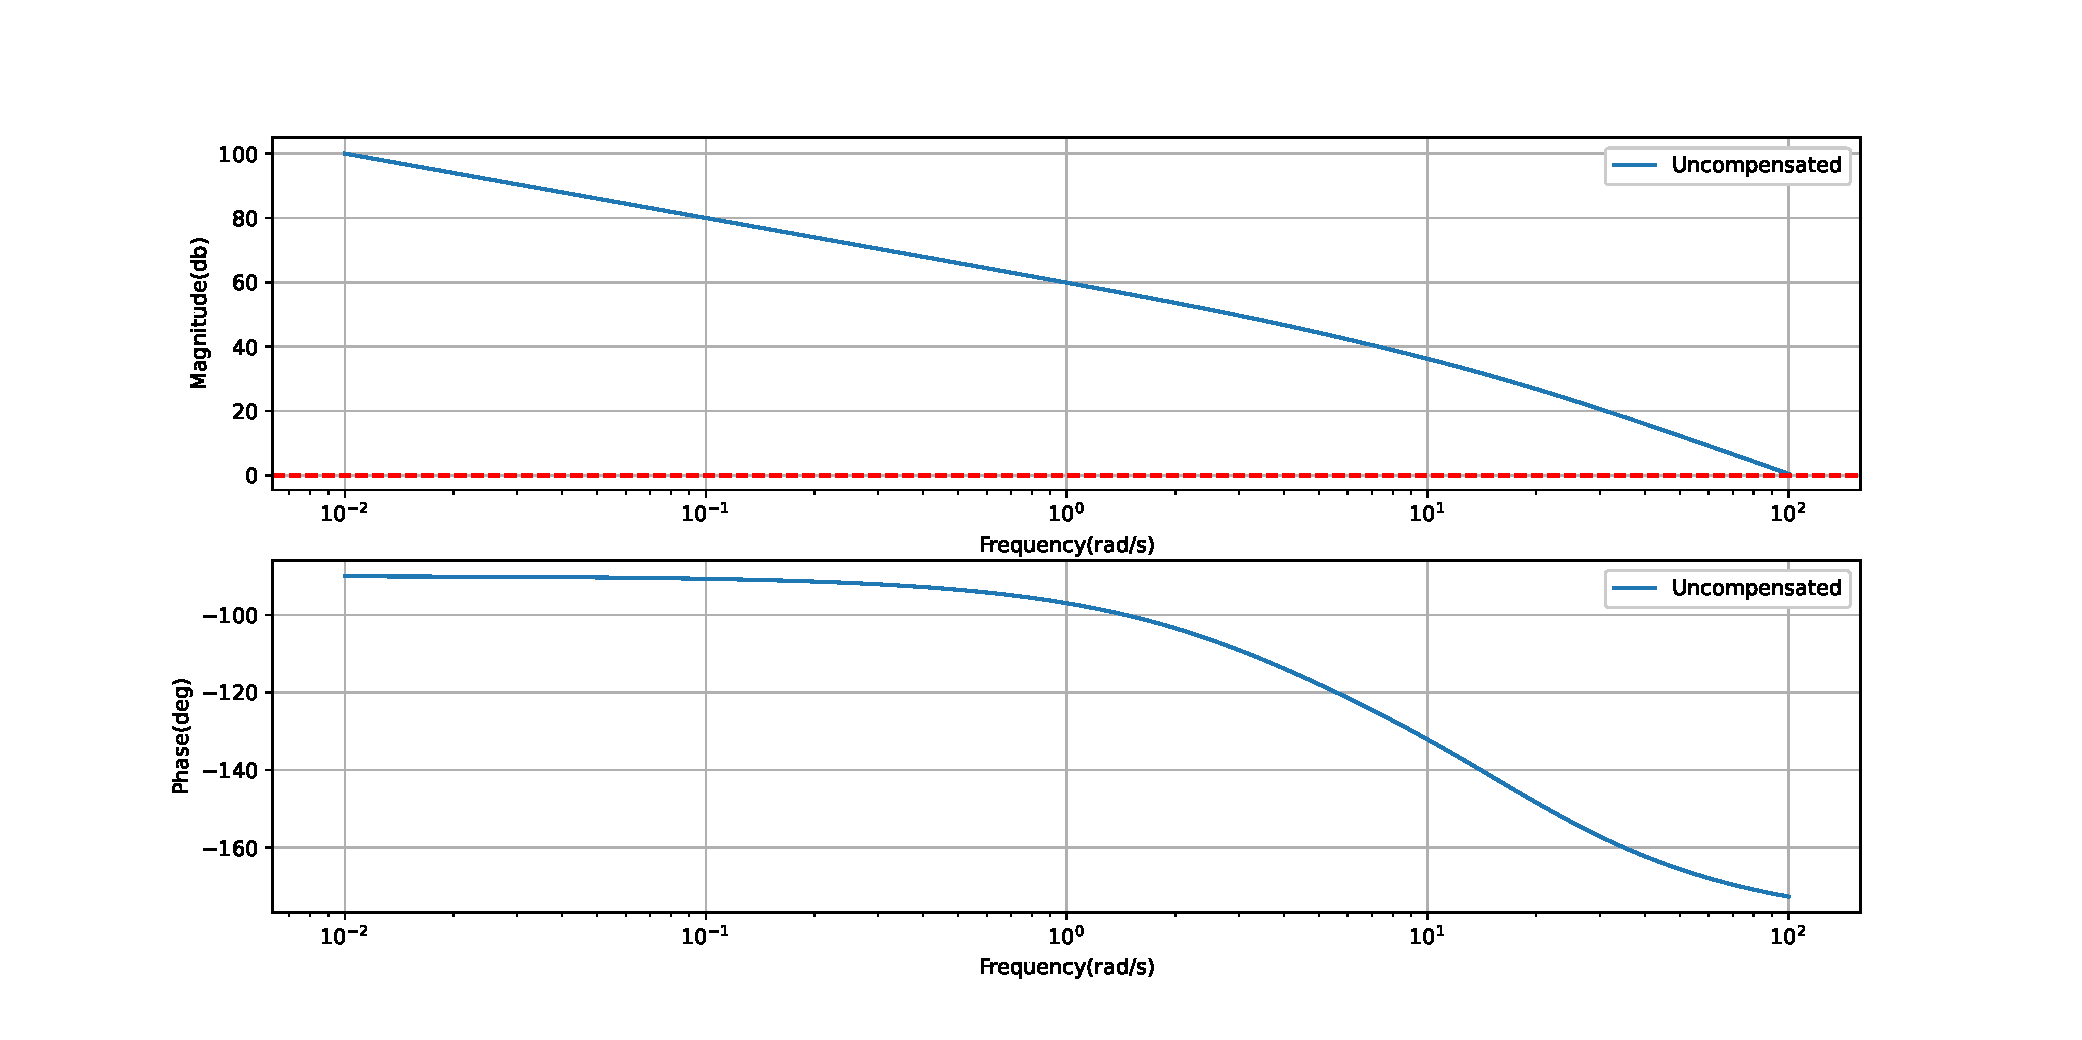
\includegraphics[width=\columnwidth]{./figs/ee18btech11012/ee18btech11012.eps}
\caption{}
\label{fig:ee18btech11012_2}
\end{figure}
%%
The following code verifies the result.
\begin{lstlisting}
codes/ee18btech11012/ee18btech11012_1.py
\end{lstlisting}
Relation between \%OS and Damping ratio
\begin{align}
\zeta &= \frac{-\ln(\%OS/100)}{\sqrt{(\pi)^2 + (\ln(\%OS/100))^2}}
\end{align}
\begin{align}
\implies\zeta &= 0.517 
\end{align}
Phase Margin for a Damping ratio is given by
\begin{align}
\phi_{m} &= 90\degree - \arctan(\frac{\sqrt{-2\zeta^2+\sqrt{1+4\zeta^4}}}{2\zeta}
\end{align}
\begin{align}
\implies \phi_{m} &= 53.17\degree
\end{align}
For an additional 5\degree for lag compensation,Phase margin is
\begin{align}
    \phi_{m} &= 53.17\degree + 5\degree= 58.17\degree
\end{align}
\textbf{Note} : Adding 5\degree phase angle to compensate the phase angle contribution of the lag compensator.
Bandwidth frequency is given by
\begin{align}
\omega_{BW} &= \omega_{n}(\sqrt{(1-2\zeta^2)+\sqrt{4\zeta^4-4\zeta^2+2}})
\end{align}
where
\begin{align}
    \omega_{n} &= \frac{4}{T_{s}\zeta}
\end{align}
Given settling time = 0.1 sec then 
\begin{align}
    \omega_{n} &= 77.37 rad/sec 
\end{align}
then
\begin{align}
    \omega_{BW} &= 96.91 rad/sec
\end{align}
\item Designing Lag-Lead Compensator Gc(s) \\
\solution 
General lag-lead compensator 
\begin{align}
G_{c}(s) &= \left(\frac{s+\frac{1}{T_1}}{s+\frac{\gamma}{T_1}}\right)\left(\frac{s+\frac{1}{T_2}}{s+\frac{1}{\gamma T_2}}\right) 
\end{align}
\begin{itemize}
\item Choose the new phase-margin frequency 
\begin{align}
    \omega_{Pm} &= 0.8 \omega_{BW} &= 77.53 rad/sec
\end{align}
\item At this phase-margin frequency,Phase angle is -170.52\degree.
\item Then the conribution required from the lead is
\begin{align}
    \phi_{max} &= 58.17-(180-170.52)=48.69\degree.
\end{align}

\item Now Using the relation 
\begin{align}
    \phi_{max} &= \sin^{-1}(\frac{1-\beta}{1+\beta})
\end{align}
then we get
\begin{align}
    \beta &= 0.142
\end{align}
\item \underline{Lag Compensator Design}:The Compensator must have a dc gain of unity to retain the value of Kv that we have already designed by setting K = 10714.
\begin{align}
    z_{clag} &= \frac{\omega_{Pm}}{10}=\frac{77.53}{10}=7.753
\end{align}
\begin{align}
    p_{clag} &= z_{clag}*\beta=1.102
\end{align}
Gain in the lag compensator is 
\begin{align}
    K_{clag} &= \frac{p_{clag}}{z_{clag}}=0.1421
\end{align}
\item Hence the lag compensator transfer function is
\begin{align}
 G_{clag}(s) &= \frac{0.1421(s+7.753)}{s+1.102} 
\end{align}
\item \underline{Lead Compensator Design}:DC gain for this must be unity.

\textbf{Relations to find T and $\beta$}:
The Compensator's magnitude at the phase margin frequency $\omega_{max}$
\begin{align}
     |G_{c}(j\omega_{max})| &= \frac{1}{\sqrt{\beta}} 
\end{align}
\begin{align}
    T &= \frac{1}{\omega_{max}\sqrt{\beta}}
\end{align}
So,To find transfer function
\begin{align}
    z_{lead} &= \frac{1}{T_{2}}=\omega_{Pm}*\sqrt{\beta}=29.92
\end{align}
\begin{align}
    p_{lead} &= \frac{z_{lead}}{\beta}=205.74,K_{lead}=\frac{p_{lead}}{z_{lead}}=7.04
\end{align}
\item Thus lead compensator transfer function is 
\begin{align}
    G_{lead} &= \frac{7.04(s+29.22)}{s+205.74} 
\end{align}
\item So the overall compensator tranfer function is
\begin{align}
    G_{c}(s) &= G_{clag}(s)G_{lead}(s)
\end{align}
\begin{align}
G_{c}(s)&=\frac{1.000384(s+7.753)(s+29.23)}{(s+1.102)(s+205.7)}
\end{align}
\end{itemize}
\item Verifying Lag-lead Compensator using Plots \\
\solution 
Magnitude and Phase plot
\begin{figure}[!ht]
\centering
  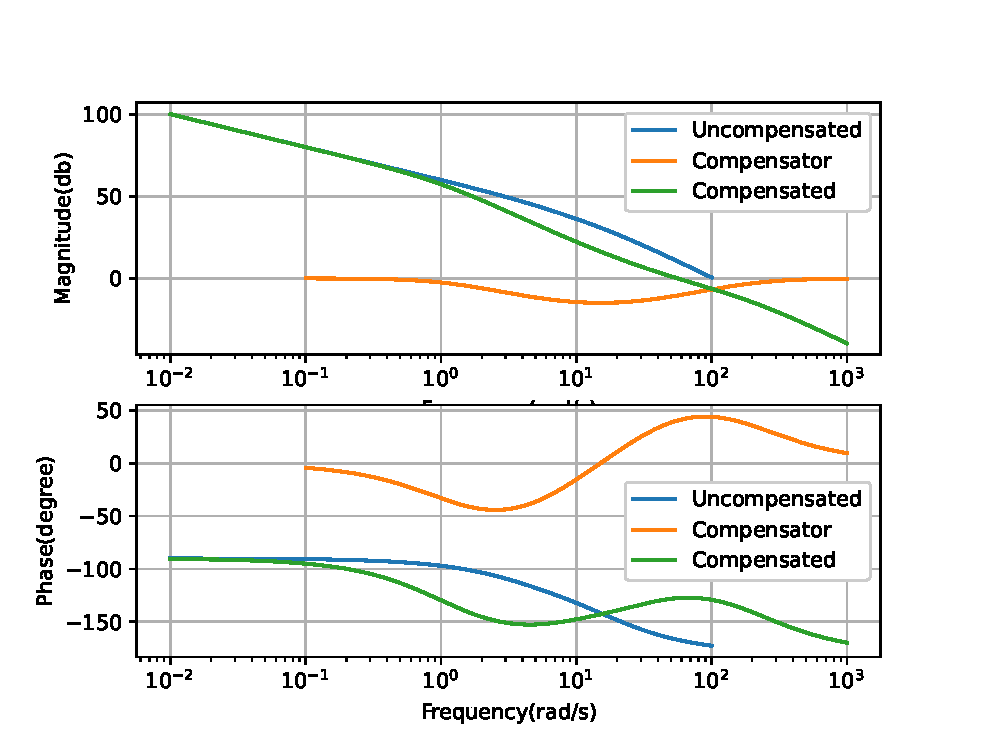
\includegraphics[width=\columnwidth]{./figs/ee18btech11012/ee18btech11012_2.eps}
\caption{}
\label{fig:ee18btech11012_3}
\end{figure}
The following code 
\begin{lstlisting}
codes/ee18btech11012/ee18btech11012_2.py
\end{lstlisting}
\item Verifying in time domain \\
\solution 
Time response for a unit step function
\begin{figure}[!ht]
\centering
  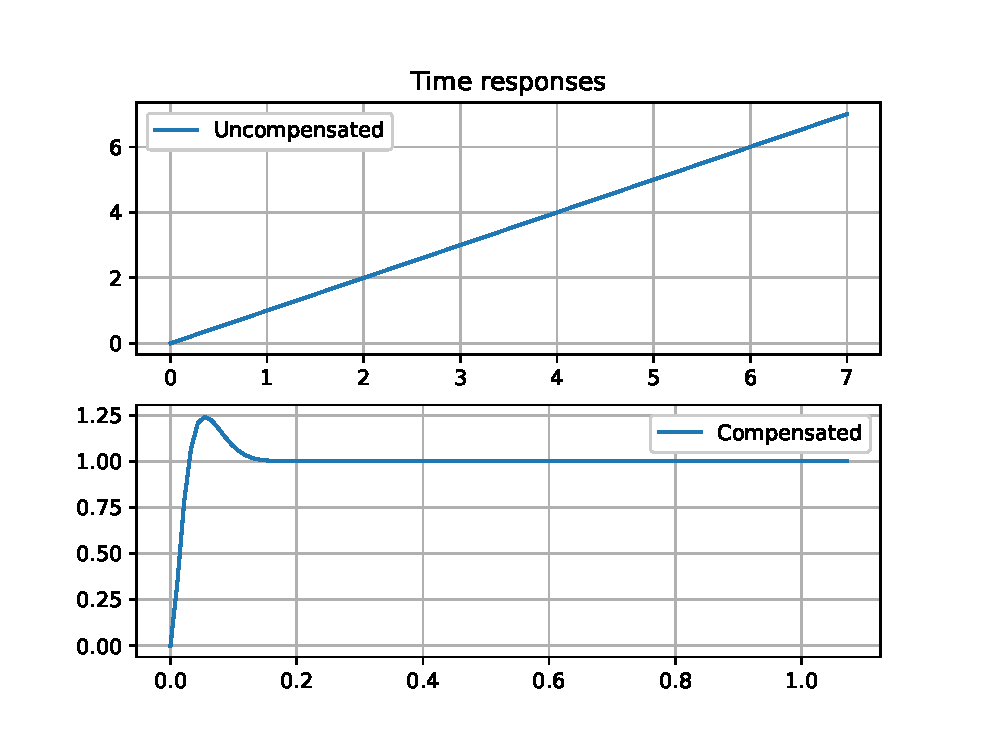
\includegraphics[width=\columnwidth]{./figs/ee18btech11012/ee18btech11012_3.eps}
\caption{}
\label{fig:ee18btech11012_4} 
\end{figure}
The following code can be verified
\begin{lstlisting}
codes/ee18btech11012/ee18btech11012_3.py
\end{lstlisting}
\item Verifying the designed lag-lead compensator \\
\solution 
\begin{table}[!ht]
\centering
%%%%%%%%%%%%%%%%%%%%%%%%%%%%%%%%%%%%%%%%%%%%%%%%%%%%%%%%%%%%%%%%%%%%%%
%%                                                                  %%
%%  This is the header of a LaTeX2e file exported from Gnumeric.    %%
%%                                                                  %%
%%  This file can be compiled as it stands or included in another   %%
%%  LaTeX document. The table is based on the longtable package so  %%
%%  the longtable options (headers, footers...) can be set in the   %%
%%  preamble section below (see PRAMBLE).                           %%
%%                                                                  %%
%%  To include the file in another, the following two lines must be %%
%%  in the including file:                                          %%
%%        \def\inputGnumericTable{}                                 %%
%%  at the beginning of the file and:                               %%
%%        \input{name-of-this-file.tex}                             %%
%%  where the table is to be placed. Note also that the including   %%
%%  file must use the following packages for the table to be        %%
%%  rendered correctly:                                             %%
%%    \usepackage[latin1]{inputenc}                                 %%
%%    \usepackage{color}                                            %%
%%    \usepackage{array}                                            %%
%%    \usepackage{longtable}                                        %%
%%    \usepackage{calc}                                             %%
%%    \usepackage{multirow}                                         %%
%%    \usepackage{hhline}                                           %%
%%    \usepackage{ifthen}                                           %%
%%  optionally (for landscape tables embedded in another document): %%
%%    \usepackage{lscape}                                           %%
%%                                                                  %%
%%%%%%%%%%%%%%%%%%%%%%%%%%%%%%%%%%%%%%%%%%%%%%%%%%%%%%%%%%%%%%%%%%%%%%



%%  This section checks if we are begin input into another file or  %%
%%  the file will be compiled alone. First use a macro taken from   %%
%%  the TeXbook ex 7.7 (suggestion of Han-Wen Nienhuys).            %%
\def\ifundefined#1{\expandafter\ifx\csname#1\endcsname\relax}


%%  Check for the \def token for inputed files. If it is not        %%
%%  defined, the file will be processed as a standalone and the     %%
%%  preamble will be used.                                          %%
\ifundefined{inputGnumericTable}

%%  We must be able to close or not the document at the end.        %%
	\def\gnumericTableEnd{\end{document}}


%%%%%%%%%%%%%%%%%%%%%%%%%%%%%%%%%%%%%%%%%%%%%%%%%%%%%%%%%%%%%%%%%%%%%%
%%                                                                  %%
%%  This is the PREAMBLE. Change these values to get the right      %%
%%  paper size and other niceties.                                  %%
%%                                                                  %%
%%%%%%%%%%%%%%%%%%%%%%%%%%%%%%%%%%%%%%%%%%%%%%%%%%%%%%%%%%%%%%%%%%%%%%

	\documentclass[12pt%
			  %,landscape%
                    ]{report}
       \usepackage[latin1]{inputenc}
       \usepackage{fullpage}
       \usepackage{color}
       \usepackage{array}
       \usepackage{longtable}
       \usepackage{calc}
       \usepackage{multirow}
       \usepackage{hhline}
       \usepackage{ifthen}



%%  End of the preamble for the standalone. The next section is for %%
%%  documents which are included into other LaTeX2e files.          %%
\else

%%  We are not a stand alone document. For a regular table, we will %%
%%  have no preamble and only define the closing to mean nothing.   %%
    \def\gnumericTableEnd{}

%%  If we want landscape mode in an embedded document, comment out  %%
%%  the line above and uncomment the two below. The table will      %%
%%  begin on a new page and run in landscape mode.                  %%
%       \def\gnumericTableEnd{\end{landscape}}
%       \begin{landscape}


%%  End of the else clause for this file being \input.              %%
\fi

%%%%%%%%%%%%%%%%%%%%%%%%%%%%%%%%%%%%%%%%%%%%%%%%%%%%%%%%%%%%%%%%%%%%%%
%%                                                                  %%
%%  The rest is the gnumeric table, except for the closing          %%
%%  statement. Changes below will alter the table's appearance.     %%
%%                                                                  %%
%%%%%%%%%%%%%%%%%%%%%%%%%%%%%%%%%%%%%%%%%%%%%%%%%%%%%%%%%%%%%%%%%%%%%%

\providecommand{\gnumericmathit}[1]{#1} 
%%  Uncomment the next line if you would like your numbers to be in %%
%%  italics if they are italizised in the gnumeric table.           %%
%\renewcommand{\gnumericmathit}[1]{\mathit{#1}}
\providecommand{\gnumericPB}[1]%
{\let\gnumericTemp=\\#1\let\\=\gnumericTemp\hspace{0pt}}
 \ifundefined{gnumericTableWidthDefined}
        \newlength{\gnumericTableWidth}
        \newlength{\gnumericTableWidthComplete}
        \newlength{\gnumericMultiRowLength}
        \global\def\gnumericTableWidthDefined{}
 \fi
%% The following setting protects this code from babel shorthands.  %%
 \ifthenelse{\isundefined{\languageshorthands}}{}{\languageshorthands{english}}
%%  The default table format retains the relative column widths of  %%
%%  gnumeric. They can easily be changed to c, r or l. In that case %%
%%  you may want to comment out the next line and uncomment the one %%
%%  thereafter                                                      %%
\providecommand\gnumbox{\makebox[0pt]}
%%\providecommand\gnumbox[1][]{\makebox}

%% to adjust positions in multirow situations                       %%
\setlength{\bigstrutjot}{\jot}
\setlength{\extrarowheight}{\doublerulesep}

%%  The \setlongtables command keeps column widths the same across  %%
%%  pages. Simply comment out next line for varying column widths.  %%
\setlongtables

\setlength\gnumericTableWidth{%
	70pt+%
	70pt+%
	70pt+%
0pt}
\def\gumericNumCols{3}
\setlength\gnumericTableWidthComplete{\gnumericTableWidth+%
         \tabcolsep*\gumericNumCols*2+\arrayrulewidth*\gumericNumCols}
\ifthenelse{\lengthtest{\gnumericTableWidthComplete > \linewidth}}%
         {\def\gnumericScale{\ratio{\linewidth-%
                        \tabcolsep*\gumericNumCols*2-%
                        \arrayrulewidth*\gumericNumCols}%
{\gnumericTableWidth}}}%
{\def\gnumericScale{1}}

%%%%%%%%%%%%%%%%%%%%%%%%%%%%%%%%%%%%%%%%%%%%%%%%%%%%%%%%%%%%%%%%%%%%%%
%%                                                                  %%
%% The following are the widths of the various columns. We are      %%
%% defining them here because then they are easier to change.       %%
%% Depending on the cell formats we may use them more than once.    %%
%%                                                                  %%
%%%%%%%%%%%%%%%%%%%%%%%%%%%%%%%%%%%%%%%%%%%%%%%%%%%%%%%%%%%%%%%%%%%%%%

\ifthenelse{\isundefined{\gnumericColA}}{\newlength{\gnumericColA}}{}\settowidth{\gnumericColA}{\begin{tabular}{@{}p{70pt*\gnumericScale}@{}}x\end{tabular}}
\ifthenelse{\isundefined{\gnumericColB}}{\newlength{\gnumericColB}}{}\settowidth{\gnumericColB}{\begin{tabular}{@{}p{70pt*\gnumericScale}@{}}x\end{tabular}}
\ifthenelse{\isundefined{\gnumericColC}}{\newlength{\gnumericColC}}{}\settowidth{\gnumericColC}{\begin{tabular}{@{}p{70pt*\gnumericScale}@{}}x\end{tabular}}

\begin{tabular}[c]{%
	b{\gnumericColA}%
	b{\gnumericColB}%
	b{\gnumericColC}%
	}

%%%%%%%%%%%%%%%%%%%%%%%%%%%%%%%%%%%%%%%%%%%%%%%%%%%%%%%%%%%%%%%%%%%%%%
%%  The longtable options. (Caption, headers... see Goosens, p.124) %%
%	\caption{The Table Caption.}             \\	%
% \hline	% Across the top of the table.
%%  The rest of these options are table rows which are placed on    %%
%%  the first, last or every page. Use \multicolumn if you want.    %%

%%  Header for the first page.                                      %%
%	\multicolumn{3}{c}{The First Header} \\ \hline 
%	\multicolumn{1}{c}{colTag}	%Column 1
%	&\multicolumn{1}{c}{colTag}	%Column 2
%	&\multicolumn{1}{c}{colTag}	\\ \hline %Last column
%	\endfirsthead

%%  The running header definition.                                  %%
%	\hline
%	\multicolumn{3}{l}{\ldots\small\slshape continued} \\ \hline
%	\multicolumn{1}{c}{colTag}	%Column 1
%	&\multicolumn{1}{c}{colTag}	%Column 2
%	&\multicolumn{1}{c}{colTag}	\\ \hline %Last column
%	\endhead

%%  The running footer definition.                                  %%
%	\hline
%	\multicolumn{3}{r}{\small\slshape continued\ldots} \\
%	\endfoot

%%  The ending footer definition.                                   %%
%	\multicolumn{3}{c}{That's all folks} \\ \hline 
%	\endlastfoot
%%%%%%%%%%%%%%%%%%%%%%%%%%%%%%%%%%%%%%%%%%%%%%%%%%%%%%%%%%%%%%%%%%%%%%

\hhline{|-|-|-|}
	 \multicolumn{1}{|p{\gnumericColA}|}%
	{\gnumericPB{\centering}\textbf{Parameter Specification}}
	&\multicolumn{1}{p{\gnumericColB}|}%
	{\gnumericPB{\centering}\textbf{Proposed}}
	&\multicolumn{1}{p{\gnumericColC}|}%
	{\gnumericPB{\centering}\textbf{Actual}}

\\
\hhline{|-|-|-|}
	 \multicolumn{1}{|p{\gnumericColA}|}%
	{\gnumericPB{\centering}Phase Margin}
	&\multicolumn{1}{p{\gnumericColB}|}%
	{\gnumericPB{\centering}53.17\degree}
	&\multicolumn{1}{p{\gnumericColC}|}%
	{\gnumericPB{\centering}53.3994\degree}
	
\\
\hhline{|-|-|-|}
	 \multicolumn{1}{|p{\gnumericColA}|}%
	{\gnumericPB{\centering}$K_{v}$}
	&\multicolumn{1}{p{\gnumericColB}|}%
	{\gnumericPB{\centering}1000}
	&\multicolumn{1}{p{\gnumericColC}|}%
	{\gnumericPB{\centering}1023.67}
\\
\hhline{|-|-|-|}
	 \multicolumn{1}{|p{\gnumericColA}|}%
	{\gnumericPB{\centering}Phase Margin frequency}
	&\multicolumn{1}{p{\gnumericColB}|}%
	{\gnumericPB{\centering}77.53}
	&\multicolumn{1}{p{\gnumericColC}|}%
	{\gnumericPB{\centering}55.5874}
	
\\

\hhline{|-|-|-|}
\end{tabular}

\ifthenelse{\isundefined{\languageshorthands}}{}{\languageshorthands{\languagename}}
\gnumericTableEnd

\caption{Comparing the desired and obtained results}
\label{table:ee18btech11012_table1}
\end{table}
\end{enumerate}
